\section{Introduction}


Due to the popularity of 3D scanners, meshes are becoming more and more accessible. However, noises from various sources are still unavoidable for many generated meshes.
Mesh filtering becomes a vital tool for denoising. It can also be used for smoothing and texture removing.
Although many mesh filters yield promising results \cite{jones2003non, zheng2011bilateral, he2013mesh, Zhang2015Filter, Wang2015rolling}, preserving various features when denoising remains a challenge.

% Mesh filtering is a kind of signal filtering for 2D manifold.
%Just like many 1D signal filters and 2D image filters,
Many traditional signal or image filters replace the signal value at each sample by a weighted average of signal values from nearby samples, and only Euclidean distance between samples is considered when computing the weight between the current sample and one of its neighbours. Such filters fail to preserve features.
The bilateral filter, introduced in \cite{tomasi1998bilateral}, is a famous edge-preserving image filter. Its weights depend not only on the spatial closeness, but also on the intensity difference.
Recently, the guided filters \cite{Petschnigg2004, he2010guided} further set the filtering weights using the intensity differences from another image and yield better edge-preservation.
Due to their success in image processing and computational photography,
researchers make many attempts expand them to mesh denoising and smoothing \cite{jones2003non, zheng2011bilateral, Solomon2014general, Zhang2015Filter}.

However, the above methods have two defects. First, choosing a large neighborhood will result in smoothed edges, while selecting a small one would limit the ability of removing noise.
Second, they can not handle close-by edges well. When there are close-by edges, samples with both close Euclidean distance and range value may come from different regions separated by another narrow region. Hence, for such sample pairs, both of them should contribute nothing to the filtering of the other one, shown in the figure~\ref{Fig:relation}.
%(\jj{an illustrative figure is needed. current figure is not good. an 1d illustration is better.})
The reason behind is that these methods compute the filtering weight between a pair of samples only using the properties of the two samples. The samples between them are ignored. Hence we wish to take the geodesic path between them into consideration to solve above problems effectively.
Although the geodesic filter~\cite{grazzini2009edge} and propagated image filter \cite{Chang2015propagated} also use the samples on the geodesic path when computing weights for superior edge-preservation. They are not expanded to mesh filtering and they do not provide a generalized model for the problem.

\begin{figure}
\centering
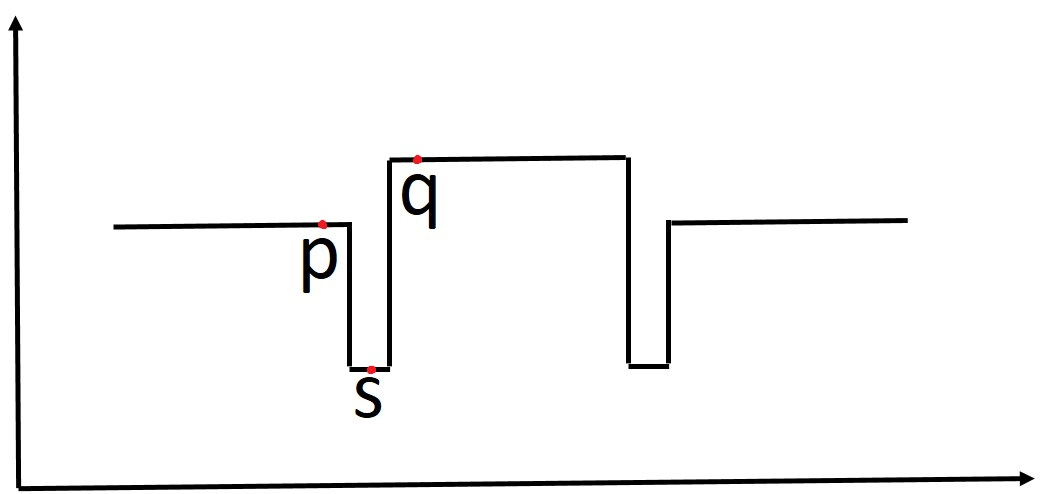
\includegraphics[width = 5.0cm]{results/Relation/relation.jpg}
\vspace{-0.5mm}
\caption{ When filtering the signals on $p$ and $q$, if the $p$ and $q$ are close and their signal values are equal, classical filters offer a large weight.
It is not reasonable. Our method solves this problem by the middle signal value on $s$. }
\label{Fig:relation}
\end{figure}

In our paper, we introduce an intrinsic filtering model for geometry signal (position, normal, curvature and so on) on 2D manifold. 
It is an universal model and many state-of-the-art filters are special cases of it, such as bilateral filter, geodesic filter and propagated filter. 
We estimate the weight between the current point and its neighbor based on the integral of the p norm of some properties' difference along the geodesic path between them, 
which yields to better edge-preservation when denoising and smoothing. 
Based on the generalized filtering model, we present a novel mesh denoising method following the common meshing denoising framework. 
The position of vertices are updated after filtering the face normals, and the two steps are iterated until achieving a satisfactory results.
However, the generation of geodesic path for each face and its neighbors during all the iterations are extremely time consuming. We design a particular pattern on each face's tangent plane to approximate the integral along the geodesic path. It is very efficient and yields even better experimental results.
Besides, considering that even geometrically complex shapes can be characterized by a rather small number of features, which means large normal differences are sparse, L1 norm is employed in the integral.
Benefiting from the intrinsic filtering model and the above two enhancements for meshes, extensive experiments illustrate the efficacy of our mesh denoising approach and it achieves more desirable results comparing with the state-of-the-art mesh denoising methods.
